\documentclass{scrbook}

%!TEX root = thesis.tex

% Set german to default language and load english as well
\usepackage[english,ngerman]{babel}

% Set UTF8 as input encoding
\usepackage[utf8]{inputenc}

% Set T1 as font encoding
\usepackage[T1]{fontenc}
% Load a slightly more modern font
\usepackage{lmodern}
% Use the symbol collection textcomp, which is needed by listings.
\usepackage{textcomp}
% Load a better font for monospace.
\usepackage{courier}

% Set some options regarding the document layout. See KOMA guide
\KOMAoptions{%
  paper=a4,
  fontsize=12pt,
  parskip=half,
  headings=normal,
  BCOR=1cm,
  headsepline,
  bibliography=openstyle,
  DIV=12}

% do not align bottom of pages
\raggedbottom

% set style of captions
\setcapindent{0pt} % do not indent second line of captions
\setkomafont{caption}{\small}
\setkomafont{captionlabel}{\bfseries}
\setcapwidth[c]{0.9\textwidth}

% set the style of the bibliography
\bibliographystyle{alpha}

% load extended tabulars used in the list of abbreviation
\usepackage{tabularx}

% load the color package and enable colored tables
\usepackage[table]{xcolor}

% define new environment for zebra tables
\newcommand{\mainrowcolors}{\rowcolors{1}{maincolor!25}{maincolor!5}}
\newenvironment{zebratabular}{\mainrowcolors\begin{tabular}}{\end{tabular}}
\newcommand{\setrownumber}[1]{\global\rownum#1\relax}
\newcommand{\headerrow}{\rowcolor{maincolor!50}\setrownumber1}

% add main color to section headers
\addtokomafont{chapter}{\color{maincolor}}
\addtokomafont{section}{\color{maincolor}}
\addtokomafont{subsection}{\color{maincolor}}
\addtokomafont{subsubsection}{\color{maincolor}}
\addtokomafont{paragraph}{\color{maincolor}}

% do not print numbers next to each formula
\usepackage{mathtools}
\mathtoolsset{showonlyrefs}
% left align formulas 
\makeatletter
\@fleqntrue\let\mathindent\@mathmargin \@mathmargin=\leftmargini
\makeatother

% Allow page breaks in align environments
\allowdisplaybreaks

% header and footer
\usepackage{scrpage2}
\pagestyle{scrheadings}
\setkomafont{pagenumber}{\normalfont\sffamily\color{maincolor}}
\setkomafont{pageheadfoot}{\normalfont\sffamily}
\setheadsepline{0.5pt}[\color{maincolor}]

% load TikZ to draw diagrams
\usepackage{tikz}

% load additional libraries for TikZ
\usetikzlibrary{%
  automata,%
  positioning,%
}

% set some default options for TikZ -- in this case for automata
\tikzset{
  every state/.style={
    draw=maincolor,
    thick,
    fill=maincolor!18,
    minimum size=0pt
  }
}

% load listings package to typeset sourcecode
\usepackage{listings}

% set some options for the listings package
\lstset{%
  numbers=none,%
  showstringspaces=false,%
  upquote=true,%
  basicstyle=\ttfamily,%
  keywordstyle=\color{keywordcolor}\slshape,%
  commentstyle=\color{commentcolor}\itshape,%
  stringstyle=\color{stringcolor},%
  mathescape=true,%
  keepspaces=true}

% load the AMS math library to typeset formulas
\usepackage{amsmath}
\usepackage{amsthm}
\usepackage{thmtools}
\usepackage{amssymb}

% load the paralist library to use compactitem and compactenum environment
\usepackage{paralist}

% load varioref and hyperref to create nicer references using vref
\usepackage[ngerman]{varioref}
\usepackage{hyperref}

% setup hyperref
\hypersetup{breaklinks=true,
            pdfborder={0 0 0},
            ngerman,
            pdfhighlight={/N},
            pdfdisplaydoctitle=true}

% define german names for referenced elements
% (vref automatically inserts these names in front of the references)
\labelformat{figure}{Abbildung\ #1}
\labelformat{table}{Tabelle\ #1}
\labelformat{appendix}{Anhang\ #1}
\labelformat{chapter}{Kapitel\ #1}
\labelformat{section}{Abschnitt\ #1}
\labelformat{subsection}{Unterabschnitt\ #1}
\labelformat{subsubsection}{Unterunterabschnitt\ #1}

% define theorem environments
\declaretheorem[numberwithin=chapter,style=plain]{Theorem}
\labelformat{Theorem}{Theorem\ #1}

\declaretheorem[sibling=Theorem,style=plain]{Lemma}
\labelformat{Lemma}{Lemma\ #1}

\declaretheorem[sibling=Theorem,style=definition]{Definition}
\labelformat{Definition}{Definition\ #1}

\declaretheorem[sibling=Theorem,style=definition]{Beispiel}
\labelformat{Beispiel}{Beispiel\ #1}

\declaretheorem[sibling=Theorem,style=definition]{Bemerkung}
\labelformat{Bemerkung}{Bemerkung\ #1}

% Use this file to define some macros you need in your thesis. A macro is a short command that inserts some mathematical symbols or texts you do not want to retype each time you need some. I recommend to use as many macros as possible, because you are able to change them later. For example if you use the same macro each time you need to give the formal semantics of an expression you can easily change the appearance of these brackets by updating the macro later on.

% Set of natural numbers
\newcommand{\N}{\mathbb{N}}

% The default epsilon does not look very nice
\let\epsilon\varepsilon

% If you need to use mathematical expressins like an epsilon in the section titles of your thesis you will end up with warnings that these special symbols cannot be included in the PDF favorites. The following macro uses the mathematical symbol during the text of the thesis and the string "Epsilon" in the PDF favorites.
\newcommand{\pdfepsilon}{\texorpdfstring{$\epsilon$}{Epsilon}}


% Set title and author used in the PDF meta data
\hypersetup{
  pdftitle={Wie schreibe ich eine Masterarbeit?},
  pdfauthor={Erika Mustermann}
}

% Depending on which of the following two color schemes you import your thesis will be in color or grayscale. I recommend to generate a colored version as a PDF and a grayscale version for printing.

%!TEX root = thesis.tex

% define color of example university
\xdefinecolor{exampleuniversity}{rgb}{1, 0.5, 0}

\colorlet{maincolor}{ForestGreen}

\colorlet{stringcolor}{green!60!black}
\colorlet{commentcolor}{black!50}
\colorlet{keywordcolor}{maincolor!80!black}

\newcommand{\imagesuffix}{-color}

%\colorlet{maincolor}{black}

\colorlet{stringcolor}{black}
\colorlet{commentcolor}{black!50}
\colorlet{keywordcolor}{black}

\newcommand{\imagesuffix}{-gray}

\newcommand{\duedate}{15. Juli 2016}

%\includeonly{pi-function}

\begin{document}
  \frontmatter
  %!TEX root = thesis.tex

\begin{titlepage}
  \thispagestyle{empty}

  \vskip1cm

  \pgfimage[height=2.5cm]{uni-logo-example\imagesuffix}
  
  \vskip2.5cm
  
  \LARGE
  
  \textbf{\sffamily\color{maincolor}Spaß mit Primzahlen}

  \textit{Primzahlen und Primfaktorzerlegung usw. usf}

  \normalfont\normalsize

  \vskip2em
  
  \textbf{\sffamily\color{maincolor}Masterarbeit}

  im Rahmen des Studiengangs \\
  \textbf{\sffamily\color{maincolor}Informatik} \\
  der Universität zu Lübeck

  \vskip1em

  vorgelegt von \\
  \textbf{\sffamily\color{maincolor}Fabian Grieser und Christian Hyttrek}

  \vskip1em
  
  ausgegeben und betreut von \\
  \textbf{\sffamily\color{maincolor}Prof. Dr. Erika Musterfrau}

  \vskip1em

  mit Unterstützung von\\
  Lieschen Müller

  \vskip1em

  Die Arbeit ist im Rahmen einer Tätigkeit bei der Firma Muster GmbH entstanden.


  \vfill

  Musterhausen, den \duedate
\end{titlepage}

  %!TEX root = thesis.tex

\cleardoublepage
\thispagestyle{plain}
\vspace*{\fill}

\section*{Erklärung}

Hiermit erkläre ich an Eides statt, dass ich die vorliegende
Arbeit ohne unzulässige Hilfe Dritter und ohne die Benutzung anderer
als der angegebenen Hilfsmittel selbständig verfasst habe;
die aus anderen Quellen direkt oder indirekt übernommenen Daten und Konzepte
sind unter Angabe des Literaturzitats gekennzeichnet.

\vskip2cm

\rule{5cm}{0.4pt}\\
(Max Mustermann)\\
Musterhausen, den \duedate

  %!TEX root = thesis.tex

\cleardoublepage
\thispagestyle{plain}

\pdfbookmark{Kurzfassung}{kurzfassung}
\paragraph{Kurzfassung}
Die Ihnen vorliegende Arbeit befasst sich mit dem hochinteressanten Themengebiet der Primzahlen. 
Eine Primzahl ist bekanntlich eine natürliche Zahl, die größer ist als 1 und nur durch sich selbst und 1 teilbar ist.
In dieser Arbeit werden Sie lesen was die Primfaktorzerlegung ist und irgendwelche Anwendungszwecke.

\cleardoublepage
\thispagestyle{plain}

\foreignlanguage{english}{%
\pdfbookmark{Abstract}{abstract}
\paragraph{Abstract} 
   The work in hand is about the marvellous topic of prime numbers. 
   A prime number is, as we all know, a natural number, which is greater than 1 and only divisable by 1 and the number itself.
   In this work you will read how the prime factorization is done and some use cases.
}


  \cleardoublepage
  \phantomsection
  \pdfbookmark{Inhaltsverzeichnis}{tableofcontents}
  \markboth{Inhaltsverzeichnis}{}
  \tableofcontents

  \mainmatter
  \chapter{Einleitung}

Die Einleitung führt zum eigentlichen Thema dieser Arbeit hin. Dabei wird ein großer Bogen gespannt, in dem die Relevanz und der Kontext der untersuchten Thematik deutlich wird. Grundlegende Begriffe aus dem Titel und der Kurzfassung sollten aufgegriffen und definiert werden. Unterstützend können Zitate herangezogen werden, die der Arbeit einen Rahmen geben.

\section{Verwandte Arbeiten}

Eine wichtiger Abschnitt der Einleitung stellt einen Überblick über verwandte Arbeiten dar. Was wurde bereits in der Literatur untersucht und ist \emph{nicht} Thema dieser Arbeit?

\section{Aufbau der Arbeit}

Neben dieser Einleitung und der Zusammenfassung am Ende gliedert sich diese Arbeit in die folgenden drei Kapitel.
\begin{description}
  \item[\ref{chapter-basics}] beschreibt die für diese Arbeit benötigten Grundlagen. In diesem Kapitel werden \ldots, \ldots und \ldots eingeführt, da diese für die folgenden Kapitel dringend benötigt werden.
  \item[\ref{chapter-konzept}] stellt das eigentliche Konzept vor. Dabei handelt es sich um ein Konzept zur Verbesserung der Welt. Das Kapitel gliedert sich daher in einen globalen und einen lokalen Ansatz, wie die Welt zum Besseren beeinflusst werden kann.
  \item[\ref{chapter-evaluation}] beinhaltet eine Evaluation des Konzeptes aus dem vorherigen Kapitel. Anhand von Simulationen wird in diesem Kapitel untersucht, wie die Welt durch konkrete Maßnahmen deutlich verbessert werden kann.
\end{description}


  \chapter{Primfaktorzerlegung}

Es gilt der Fundamentalsatz der Arithmetik: Jede positive ganze Zahl lässt sich als Produkt von Primzahlen darstellen, und diese Darstellung ist bis auf die Reihenfolge der Primzahlen eindeutig\cite{scala}. 
Diese Primzahlen nennt man die Primfaktoren der Zahl. 
Man kennt bisher keine Methode, um die Primfaktorzerlegung einer beliebigen gegebenen Zahl effizient zu bestimmen, d. h. in einer Zeit, die polynomiell mit der Länge der Zahl wächst. 
Die Faktorisierungsannahme besagt, dass es eine solche Methode auch nicht gibt. 
Man versucht, die Zeit mit geeigneten Faktorisierungsverfahren zu minimieren.

Aufgrund dieses Satzes, also dass sich jede natürliche Zahl größer 0 durch Multiplikation von Primzahlen eindeutig darstellen lässt, nehmen die Primzahlen eine besondere atomare Stellung in der Mathematik ein\cite{rltl}.
Alexander K. Dewdney bezeichnete diese als den Elementen der Chemie weitgehend ähnlich.

In \vref{fig:tolleAbbildung} sehen Sie eine schematische Darstellung der Primfaktorzerlegung.

\begin{figure}[h]
    \centering
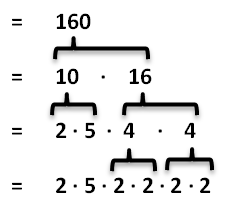
\includegraphics[width=0.5\linewidth]{primeFac.png}

    \caption{Eine super Abbildung}
    \label{fig:tolleAbbildung}
\end{figure}


  \chapter{Pi-Funktion und Primzahlsatz}

Zur Untersuchung der Verteilungen der Primzahlen betrachtet man unter anderem die Funktion

\begin{equation*}
    \pi:\mathbb{N} \rightarrow \mathbb{N}, n \mapsto \pi(n)
\end{equation*}
die die Anzahl der Primzahlen $\leq n$ angibt und auch \emph{Primzahlzählfunktion} genannt wird.
Z.B. ist 

\begin{equation*}
    \pi(1)=0;\quad \pi(10)=4;\quad \pi(100)=25; \quad \pi(1000)=168;\quad \pi(1000000)=78498
\end{equation*}

Diese Funktion und ihr Wachstumsverhalten ist ein beliebter Forschungsgegenstand in der Zahlentheorie.
Mit der Zeit wurden einige Näherungsformeln entwickelt und verbessert \cite{MopOverview}

Der Primzahlsatz besagt, dass

\begin{equation*}
    \pi(x)\sim\frac x {\ln x}
\end{equation*}

gilt, das heißt, dass der Quotient von linker und rechter Seite für $x \rightarrow \infty$ gegen 1 strebt:

\begin{equation*}
    \lim_{x \rightarrow \infty}\frac{\pi(x)}{\frac{x}{\ln x}}=1
\end{equation*}


\begin{figure}[h]
    \centering
    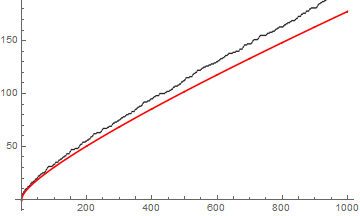
\includegraphics[width=0.5\linewidth]{pi-func.png}
    \caption{Die Pi-Funktion}
    \label{fig:pi-function}
\end{figure}




  \chapter{Zusammenfassung}
In der Ringtheorie wird das Konzept der Primzahl auf die Elemente eines beliebigen kommutativen unitären Rings verallgemeinert. Die entsprechenden Begriffe sind Primelement und irreduzibles Element.

Die Primzahlen und deren Negative sind dann genau die Primelemente und auch genau die irreduziblen Elemente des Rings der ganzen Zahlen. In faktoriellen Ringen, das sind Ringe mit eindeutiger Primfaktorisierung, fallen die Begriffe Primelement und irreduzibles Element zusammen; im Allgemeinen ist die Menge der Primelemente jedoch nur eine Teilmenge der Menge der irreduziblen Elemente.

Insbesondere im zahlentheoretisch bedeutsamen Fall der Dedekindringe übernehmen Primideale die Rolle der Primzahlen.


  \appendix

  %!TEX root = thesis.tex

\chapter{Anhang}

Dieser Anhang enthält tiefergehende Informationen, die nicht zur eigentlichen Arbeit gehören.

\section{Abschnitt des Anhangs}

In den meisten Fällen wird kein Anhang benötigt, da sich selten Informationen ansammeln, die nicht zum eigentlichen Inhalt der Arbeit gehören. Vollständige Quelltextlisting haben in ausgedruckter Form keinen Wort und gehören daher weder in die Arbeit noch in den Anhang. Darüber hinaus gehören Abbildungen bzw. Diagramme, auf die im Text der Arbeit verwiesen wird, auf keinen Fall in den Anhang.

  \backmatter

  \cleardoublepage
  \phantomsection
  \pdfbookmark{Abbildungsverzeichnis}{listoffigures}
  \listoffigures

  \cleardoublepage
  \phantomsection
  \pdfbookmark{Tabellenverzeichnis}{listoftables}
  \listoftables

  \cleardoublepage
  \phantomsection
  \pdfbookmark{Definitions- und Theoremverzeichnis}{listoftheorems}
  \renewcommand{\listtheoremname}{Definitions- und Theoremverzeichnis}
  \listoftheorems[ignoreall,show={Lemma,Theorem,Korollar,Definition}]

  %!TEX root = thesis.tex

\cleardoublepage
\phantomsection
\pdfbookmark{Abkürzungsverzeichnis}{abbreviations}
\chapter*{Abkürzungsverzeichnis}
\label{section-abbrevs}

\begin{tabularx}{\textwidth}{lX}
  ABA & alternierender Büchi-Automat, engl. \emph{a}lternating \emph{B}üchi \emph{a}utomaton\\
  AFA & alternierender endlicher Automat, engl. \emph{a}lternating \emph{f}inite \emph{a}utomaton\\
  BA & Büchi-Automat, engl. \emph{B}üchi \emph{a}utomaton\\
  BNF & Normalform kontextfreier Grammatiken, engl. \emph{B}ackus--\emph{N}aur \emph{f}orm\\
  DFA & endlicher Automat, engl. \emph{d}eterministic \emph{f}inite \emph{a}utomaton
\end{tabularx}


  \cleardoublepage
  \phantomsection
  \pdfbookmark{Literaturverzeichnis}{bibliography}
  \bibliography{literature}
\end{document}
